% !TeX spellcheck = de_CH
% /*
%  * ----------------------------------------------------------------------------
%  * "THE BEER-WARE LICENSE" (Revision 42):
%  * <michi.wieland@hotmail.com> wrote this file. As long as you retain this notice you
%%  * can do whatever you want with this stuff. If we meet some day, and you think
%  * this stuff is worth it, you can buy me a beer in return. Michael Wieland
%  * ----------------------------------------------------------------------------
%  */

\documentclass[
a4paper,
oneside,
10pt,
fleqn,
headsepline,
toc=listofnumbered, 
bibliography=totocnumbered]{scrartcl}

% deutsche Trennmuster etc.
\usepackage[T1]{fontenc}
\usepackage[utf8]{inputenc}
\usepackage[english, ngerman]{babel} % \selectlanguage{english} if  needed
\usepackage{lmodern} % use modern latin fonts

% Custom commands
\newcommand{\AUTHOR}{Michael Wieland}
\newcommand{\INSTITUTE}{Hochschule für Technik Rapperswil}
\newcommand{\GITHUB}{https://github.com/michiwieland/hsr-zusammenfassungen}
\newcommand{\LICENSEURL}{https://en.wikipedia.org/wiki/Beerware}
\newcommand{\LICENSE}{
"THE BEER-WARE LICENSE" (Revision 42):
<michi.wieland@hotmail.com> wrote this file. As long as you retain this notice you
can do whatever you want with this stuff. If we meet some day, and you think
this stuff is worth it, you can buy me a beer in return. Michael Wieland	
}

% Jede Überschrift 1 auf neuer Seite
\let\stdsection\section
\renewcommand\section{\clearpage\stdsection}

% Multiple Authors
\usepackage{authblk}

% Include external pdf
\usepackage{pdfpages}

% Layout / Seitenränder
\usepackage{geometry}

% Inhaltsverzeichnis
\usepackage{makeidx} 
\makeindex

\usepackage{url}
\usepackage[pdfborder={0 0 0}]{hyperref}
\usepackage[all]{hypcap}
\usepackage{hyperxmp} % for license metadata

% Glossar und Abkürzungsverzeichnis
\usepackage[acronym,toc,nopostdot]{glossaries}
\glossarystyle{altlist}
\usepackage{xparse}
\DeclareDocumentCommand{\newdualentry}{ O{} O{} m m m m } {
	\newglossaryentry{gls-#3}{
		name={#4 : #5},
		text={#5\glsadd{#3}},
		description={#6},
		#1
	}
	\makeglossaries
	\newacronym[see={[Siehe:]{gls-#3}},#2]{#3}{#4}{#5\glsadd{gls-#3}}
}
\makeglossaries

% Mathematik
\usepackage{amsmath}
\usepackage{amssymb}
\usepackage{amsfonts}
\usepackage{enumitem}

% Images
\usepackage{graphicx}
\graphicspath{{images/}} % default paths

% Boxes
\usepackage{fancybox}

%Tables
\usepackage{tabu}
\usepackage{booktabs} % toprule, midrule, bottomrule
\usepackage{array} % for matrix tables

% Multi Columns
\usepackage{multicol}

% Header and footer
\usepackage{scrlayer-scrpage}
\setkomafont{pagehead}{\normalfont}
\setkomafont{pagefoot}{\normalfont}
\automark*{section}
\clearpairofpagestyles
\ihead{\headmark}
\ohead{\AUTHOR}
\cfoot{\pagemark}

% Pseudocode
\usepackage{algorithmic}
\usepackage[linesnumbered,ruled]{algorithm2e}

% Code Listings
\usepackage{listings}
\usepackage{color}
\usepackage{beramono}

\definecolor{bluekeywords}{rgb}{0,0,1}
\definecolor{greencomments}{rgb}{0,0.5,0}
\definecolor{redstrings}{rgb}{0.64,0.08,0.08}
\definecolor{xmlcomments}{rgb}{0.5,0.5,0.5}
\definecolor{types}{rgb}{0.17,0.57,0.68}

\lstdefinestyle{visual-studio-style}{
	language=[Sharp]C,
	columns=flexible,
	showstringspaces=false,
	basicstyle=\footnotesize\ttfamily, 
	commentstyle=\color{greencomments},
	morekeywords={partial, var, value, get, set},
	keywordstyle=\bfseries\color{bluekeywords},
	stringstyle=\color{redstrings},
	breaklines=true,
	breakatwhitespace=true,
	tabsize=4,
	numbers=left,
	numberstyle=\tiny\color{black},
	frame=lines,
	showspaces=false,
	showtabs=false,
	escapeinside={£}{£},
}

\definecolor{DarkPurple}{rgb}{0.4, 0.1, 0.4}
\definecolor{DarkCyan}{rgb}{0.0, 0.5, 0.4}
\definecolor{LightLime}{rgb}{0.3, 0.5, 0.4}
\definecolor{Blue}{rgb}{0.0, 0.0, 1.0}

\lstdefinestyle{cevelop-style}{
	language=C++,  
	columns=flexible,
	showstringspaces=false,     
	basicstyle=\footnotesize\ttfamily, 
	keywordstyle=\bfseries\color{DarkPurple},
	commentstyle=\color{LightLime},
	stringstyle=\color{Blue}, 
	escapeinside={£}{£}, % latex scope within code      
	breaklines=true,
	breakatwhitespace=true,
	showspaces=false,
	showtabs=false,
	tabsize=4,
	morekeywords={include,ifndef,define},
	numbers=left,
	numberstyle=\tiny\color{black},
	frame=lines,
}

\lstdefinestyle{eclipse-style}{
	language=Java,  
	columns=flexible,
	showstringspaces=false,     
	basicstyle=\footnotesize\ttfamily, 
	keywordstyle=\bfseries\color{DarkPurple},
	commentstyle=\color{LightLime},
	stringstyle=\color{Blue}, 
	escapeinside={£}{£}, % latex scope within code      
	breaklines=true,
	breakatwhitespace=true,
	showspaces=false,
	showtabs=false,
	tabsize=4,
	morekeywords={length},
	numbers=left,
	numberstyle=\tiny\color{black},
	frame=lines,
}
\lstset{style=eclipse-style}



% Theorems \begin{mytheo}{title}{label}
\usepackage{tcolorbox}
\tcbuselibrary{theorems}
\newtcbtheorem[number within=section]{definiton}{Definition}%
{fonttitle=\bfseries}{def}
\newtcbtheorem[number within=section]{remember}{Merke}%
{fonttitle=\bfseries}{rem}
\newtcbtheorem[number within=section]{hint}{Hinweis}%
{fonttitle=\bfseries}{hnt}

% Dokumentinformationen
\newcommand{\SUBJECT}{Zusammenfassung}
\newcommand{\TITLE}{Software Engineering 2}

\loadglsentries{glossar}

% pdf metadata
\hypersetup{
	pdfauthor={\AUTHOR},
	pdftitle={\SUBJECT \TITLE},
	pdfcopyright={\LICENSE},
	pdflicenseurl={\LICENSEURL}
}

\begin{document}
	
% Front page
\title{\TITLE}
\subject{\SUBJECT}
\author{\AUTHOR}
\affil{\INSTITUTE}
\date{\today}
\maketitle

\vfill

% Participate
\paragraph{Mitmachen} \hfill \\
Falls Du an diesem Dokument mitarbeiten willst, kannst Du das Dokument
auf GitHub unter \url{\GITHUB} forken.

% Licence
\paragraph{Lizenz} \hfill \\
\LICENSE

% Table of contents
\tableofcontents


% Glossar and acronyms (if included \loadglsentries{glossar})
\printglossary[type=\acronymtype]
\printglossary
\glsaddall


\section{Projektplanung}

\subsection{Meilensteine und Zwischenresultate}

\subsubsection{Messbare Zwischenresultate}

\begin{itemize}
\item Anzahl Seiten Requirements
\item Anzahl Items (Teil-Abschnitte, aufgezählte Punkte) in den nicht-funktionalen Anforderungen
\item Anzahl Klassen im Domainmodell
\item Anzahl User Stories (im Backlog, completed...)
\item Development speed (Anzahl Story Points per Sprint; bei Scrum)
\item Anzahl \& Schwere der offenen Bugs, durchschnittl. Verweildauer, Abarbeitungsgeschwindigkeit
\item Anzahl screens (GUI-Entwürfe)
\item Alle Code-Metriken (lines of code, Anzahl Klassen, Methoden, Kopplung, etc...)
\item Anzahl (nicht)erfüllte Testfälle
\item Anzahl Schnittstellen zu Umsystemen, inkl. Komplexitäts-Einschätzung S, M, L, XL
\end{itemize}
\subsection{Dokumentationen in Software Projekten}

\subsubsection{Kundensichtbarkeit von Dokumentationen}

\begin{figure}[h]
	\centering
	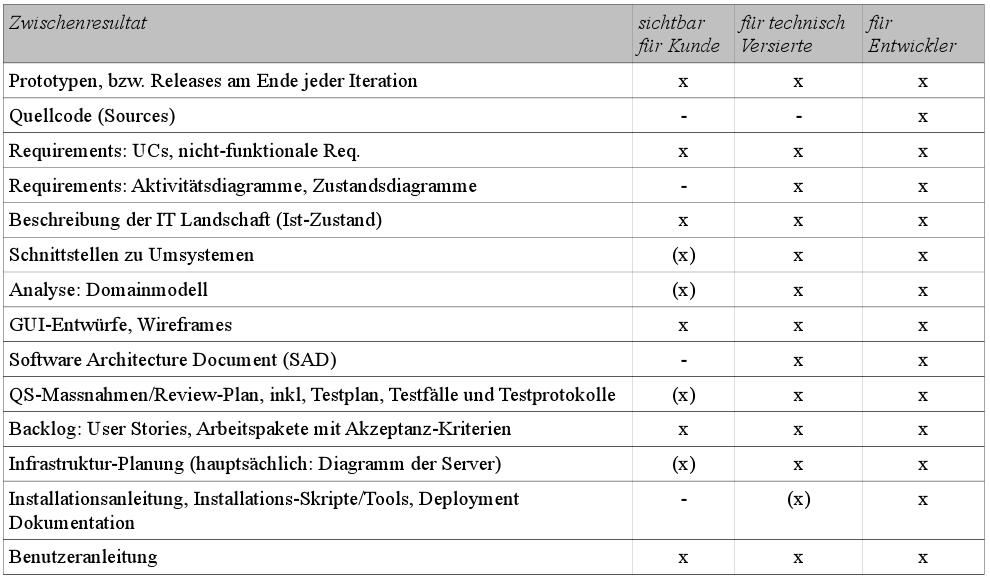
\includegraphics[width=0.9\linewidth]{img/dokumentationen_abgaben_kunde}
	\caption{Kundensichtbarkeit von Dokumentationen}
	\label{fig:dokumentationenabgabenkunde}
\end{figure}

\section{Automation}

\subsection{Build Tools}

\paragraph{Pros:} 
\begin{itemize}
	\item Automated, non-interactive process
	\item Repeatable!
	\item Independent of your IDE
	\item Time-consuming tasks can be scheduled
\end{itemize}

\paragraph{Cons:}
\begin{itemize}
	\item Automated, non-interactive process
	\item Maintenance and extension is difficult
	\item Most likely platform-dependent (.sh, .bat, ...)
\end{itemize}

\paragraph{Benefits:}
\begin{itemize}
	\item Reduce repetitive tasks
	\item Independence of any IDE
	\item Reproducible results
	\item Save time
	\item Basis for continuous integration!
\end{itemize}

\paragraph{Features / Wishlist:}
\begin{itemize}
	\item Single command builds (CRISP)
		\begin{itemize}
			\item Complete: Das Programm lässt sich bei jeder Ausführung komplett builden. 
			\item Repeatable: Wiederholbar auch für auf älteren Versionen/Tags
			\item Informative: Feedback, sprechender Output bei jedem Step 
			\item Schedulable: Planbar
			\item Portable: Plattformunabhängig ausführbar
		\end{itemize}
	\item Flexibility (run individual tasks)
	\item Performance Extensibility
\end{itemize}

\subsubsection{Make}

Imperatives Build Script, welches als DAG (Azyklischer Graph) umgesetzt wurde. Make ist plattformabhängig und hat kein Dependency Management.


\subsubsection{Ant}

Ant ist ein imperatives Build Tool mit folgenden Konzepten:
\begin{itemize}
	\item XML-based “scripting” with built-in tasks (mkdir, jar, condition,...)
	\item Focus on portability
	\item Custom tasks can be written in Java
\end{itemize}

\subsubsection{Maven}

Maven is a deklarativ build tool, designed for consistency and automated dependency management.

\paragraph{Concepts:}
\begin{itemize}
	\item Declarative (XML-based)
	\item “Convention over configuration” => Default build => Only specify differences
	\item Predefined lifecycles = DAG
	\item Default = build and deployment
	\item Clean
	\item Site = generate documentation
	\item Predefined directory tree
	\item Automated dependency resolution
\end{itemize}

\paragraph{Pros:}
\begin{itemize}
	\item More concise => shorter build-files
	\item Reusable build-logic (plug-ins)
	\item Automated dependency management (!)
\end{itemize}

\paragraph{Cons:}
\begin{itemize}
	\item Less general and flexible than “imperative” tools
	\item Impose a somewhat rigid project / file structure
\end{itemize}

\begin{figure}[h!]
	\centering
	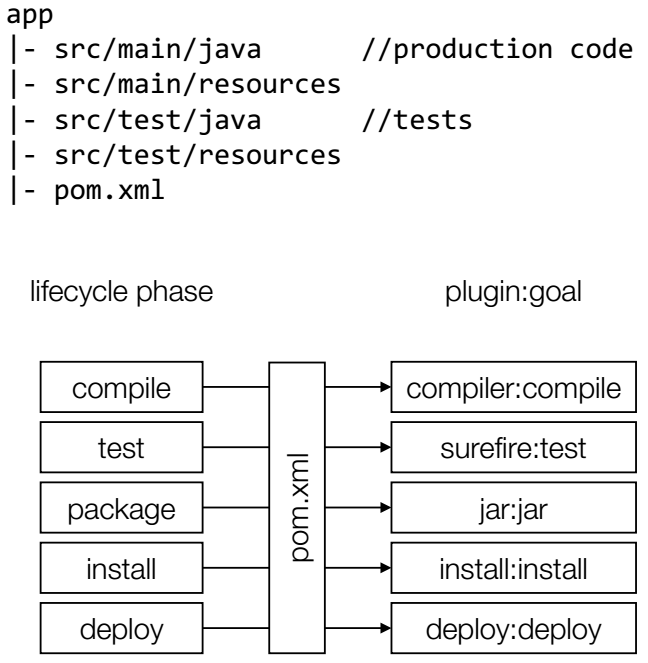
\includegraphics[width=0.5\linewidth]{img/maven_filestructure_lifecycle}
	\caption{Maven Filestructure und Lifecyle}
	\label{fig:mavenfilestructurelifecycle}
\end{figure}

\newpage


\subsection{Continuous Integration}
Continuous Integration darf nicht mit Continuous Delivery verwechselt werden! Continuous Integration beschreibt den Prozess des fortlaufenden Erstellens von Software aus mehreren Komponenten. Es stellt die Basis für Continuous Delivery dar, wobei bei Continuous Delivery die getestete Software in sehr kurzen Zyklen auf die produktiven Server deployed wird.

\subsubsection{Best Practices}
\begin{enumerate}
	\item Maintain a single source repository 
	\item Automate the build 
	\item Make the build self-testing 
	\item Everyone commits to the mainline every day 
	\item Every commit to the mainline should be built 
	\item Keep the build fast 
	\item Test in a clone of the production environment 
	\item Make it easy to get the latest deliverables 
	\item Everyone can see what’s happening 
	\item Automate deploymentMave
\end{enumerate}


\section{SE Practices}

\subsection{Requirements Practices}

\begin{itemize}
	\item Anforderungen aus Benutzersicht
	\item Kritisches Hinterfragen: Nach Grund und Ursprung für einen Wunsch Fragen.
	\item Genügend generell und Abstrakt definieren. Abstraktionsgrad sollte so hoch sein, dass der Programmierer eine konfigurierbare Lösung implementiert. 
	\item Verfolgung des Ursprungs: Person, Grund, Datum.
\end{itemize}

\subsubsection{Vorgehen}

\begin{enumerate}
	\item Dig for Requirements: Ermittlungstechniken: 
		\begin{itemize}
			\item Dokumentenstudium
			\item Befragung: Interview, Fragebogen, Workshop, Prototyp Review
			\item Beobachtung: Feldbeobachtung, Apprenticing, Bestehender Business Prozess analysieren
			\item Kreativität: Brainstorming
		\end{itemize}
	\item Make Quality a Requirement
		\begin{itemize}
			\item Qualität als (NF-)Requirements aufnehmen
				\begin{itemize}
					\item Performance, Scalability, Security, robustness
				\end{itemize}
			\item Möglichst testbare Qualitätsanforderungen
				\begin{itemize}
					\item Max. Antwortzeiten unter definierten Umständen
					\item Min. Unterstützte Datenmenge
					\item Prüfung von Daten/Geräte und Verhalten bei Fehler
				\end{itemize}
			\item Basierend auf echten Anforderungen
				\begin{itemize}
					\item Konkrete Benutzer-Erwartungen / harte externe Limiten
					\item Quantitative Werte unter definierten Rahmenbedingungen.
				\end{itemize}
			\item Qualitätsanforderungen sollten quantitativ, prägnant beschrieben werden, um Fehlinterprätationen zu verhindern.
			\item Schwieriger zu ermitteln sind unbewusste Wünsche. Diese müssen mit prägnanten Fragen gefunden werden.
			\item Von der geforderten Qualität hängen Architekturentscheide ab. Muss die Architektur während dem Projektverlauf angepasst werden, geht das ins Geld. Deshalb früh Qualitätsanforderungen prüfen.
		\end{itemize}
	\item Deal with Changes: Mythos ''Stabile Requirements''
		\begin{itemize}
			\item Ca. 2\% ändern sich pro Monat!
			\item Requirement-Änderungen Antizipieren: Details nachfragen \& abstrakt definieren
			\item Design for Change
			\item Kurze Iteration mit User-Feedback
			\item Change Assessment: Qualität nach jeder Iteration prüfen.
		\end{itemize}
\end{enumerate}


\subsection{Design Practices}

\subsubsection{Don't repeat yourself}

Repetition von Information vermeiden, damit keine Inkonsistenzen bei Änderungen entstehen:

\begin{itemize}
	\item Code Duplikationen: Logiken, Daten, Boilder-Plate Code etc.
	\item Dokumentation in Code: Redundante Beschreibungen
	\item Dokumentation separat zum Code: Wiederholung
	\item Wiederholung wegen Programmiersprache
\end{itemize}


\paragraph{DRY Techniken:}
\begin{itemize}
	\item Konstanten statt literale Konstantenwerte
	\item Vermeiden von Code-Snippets
	\item Code-Kommentare geben nur relevante Zusatzinformationen
	\item Externe Konfigurationsdaten
	\item Code-Generierung: Evtl. mit DSL (auch selbstgebaute)
\end{itemize}

\subsubsection{Archieve orthogonality}

Ziel: Hohe Kohäsion / Tiefe Kopplung. Man spricht von Orthogonalität, wenn zwei Dinge, die nichts miteinander zu tun haben, voneinander unabhängig sind. Vorteile Orthogonalität:
\begin{itemize}
	\item Selektive Wiederverwendung eines Aspekts
	\item Ein Aspekt isoliert änderbar
	\item Einfacher zu verstehen
	\item Einfacher zu testen
\end{itemize}

Zur Reduktion der Kopplung:
\begin{itemize}
	\item Hierarchische Zerlegung der Komponenten (System, Packages). Allenfalls Information Hiding, um die Verständlichkeit des Architekturdiagramms zu gewährleisten.
	\item Reduzierte Abhängigkeiten zwischen Komponenten (DAG/Keine Zyklen, Abtrennung Daten und Routinen, Kein Spaghetti Code)
\end{itemize}


\subsubsection{Design to test}

Testbarkeit vor Entwicklungszeit betrachten, hat Einfluss auf die Architektur. Schlüsselwörter:
	\begin{itemize}
	\item Klare Interfaces und Kontrakte
	\item Überlegung der relevanten Testfälle
	\item Grad der Unit-Testbarkeit und Integration-Testbarkeit
	\item Evtl. Freiheitsgrade für «Dependency Injection»
		\begin{itemize}
			\item Erzeugung und Initialisierung von benötigten Objekte ausserhalb des Benutzer Objektes (Wie Strategie Muster oder Fabrik Muster)
			\item Isoliertes Testen mit anderen Komponenten («Fakes»)
			\item Kann Design komplexer als (produktiv) nötig machen
		\end{itemize}
\end{itemize}


Schlüsselwörter:
\begin{description}
	\item[Fake] Vereinfachte Implementierung
	\item[Mock] Auf Testfall zugeschnitten; prüft Reihenfolge und Inhalt der erwarteten Aufrufe
	\item[Stub] Auf Testfall zugeschnittene Antworten
	\item[Dummy] Objekte, die nur herumgereicht, aber nie inspiziert werden.
\end{description}

\subsection{Implementation Practices}

\subsubsection{Fix broken windows}

Probleme beheben, wenn sie entstehen (kleine sofort beheben, grössere markieren und später beheben). Probleme können gut durch Refactoring erkannt werden. Refactoring beschreibt den Prozess, des Code verbesserns, ohne die Funktionalität zu verändern.

\subsubsection{Refactor early and often}

\begin{itemize} 
	\item Konstanter Verbesserungsprozess in einem wachsenden Software-Projekt
	\item Liste über die zu verbesserenden Bereichen führen
	\item Vorgehen:
		\begin{itemize}
			\item Refactoring soll keine neuen Funktionen bieten
			\item Gute Tests vor Beginn des Refactoring haben
			\item Mehrere kleinere Schritte statt einer Riesenänderung.
		\end{itemize}
\end{itemize}

\subsubsection{Program deliberately}

Gezieltes programmieren:
\begin{itemize}
	\item Klares Ziel und Design
	\item Logisch rigoros analysieren, entwickeln und testen
	\item Nur auf spezifizierte Features von Libraries verlassen
	\item Eingesetzte Technologie beherrschen
	\item Annahmen dokumentieren und mit Assert \& Tests prüfen
	\item Crash early: Alle ungültige Zustände sollen Fehler erzeuge
	\item Exceptions richtig behandeln, nicht blind unterdrücken
	\item Debugging: Auf Grund gehen, Fehler verstehen
\end{itemize}


\subsection{Verification Practices}

Verifikation besteht aus zwei Komponenten:
\begin{itemize}
	\item Statische Analyse
		\begin{itemize}
			\item Design Reviews
			\item Code Reviews
		\end{itemize}
	\item Testing (Dynamisch)
		\begin{itemize}
			\item Unit Tests
			\item Integration Tests
		\end{itemize}
\end{itemize}

\subsubsection{Test rigorously}
\begin{itemize}
	\item Früh, häufig und automatisch testen.
	\item Für gefundene Fehler sollte immer ein Test geschrieben werden, um diesen in Zukunft zu vermeiden.
	\item Integrationstests sind mindestens so wichtig wie Unit-Tests!
	\item TDD und die dadurch resultierende hohe Test Coverage ist anzustreben.
	\item Nur weil Tests existieren, sollte rigoroses Überlegen beim Programmieren nicht vernachlässigt werden. Auch 100\% Korrektheit bedeutet noch keine Korrektheit.
\end{itemize}


\subsubsection{Perform reviews}
\begin{itemize}
	\item Formale Inspektionen durchführen: Durch Experten, sowie durch Entwicklern Design \& Code Reviews. Immer festhalten der Ergebnisse (severity, Action, Verantwortlicher)
	\item Das Ziel der Reviews nicht aus den Augen verlieren: Defekte zu finden. (keine Stil oder Architekturdiskussionen)
\end{itemize}

\section{Test Driven Development}
The TDD way to write code is to write tests that don't pass, then make them pass.
\begin{enumerate}
	\item Red: Schreibe zuerst einen Test, der fehlschlägt, weil das geforderte Feature noch nicht umgesetzt ist. (er sollte aber kompilieren) %TODO: Wirklich? D.h. Klassen/Interfaces müssen bereits erstellt werden?
	\item Green:  Ändere den Code bis der Test durchläuft
	\item Refactor: Refactore den Code sowie den Microtest bis diese ein kosistentes, gutes Design aufweisen. 
	\item Integrate (optional): Der geschriebene Code und Tests in die Codebase einfügen. Dieser Schritt kann auch von einem CI-System übernommen werden.
\end{enumerate}

\begin{figure}[h!]
	\centering
	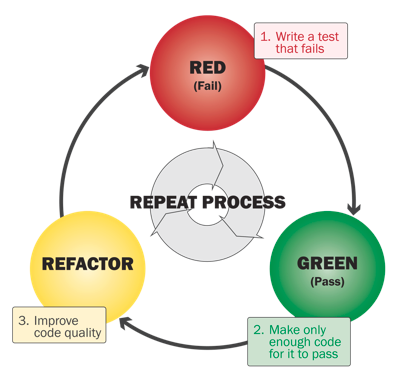
\includegraphics[width=0.5\linewidth]{img/tdd_cycle}
	\caption{TDD Lifecycle}
	\label{fig:tddcycle}
\end{figure}

\subsection{Produktivität}
TDD verbessert wegen den folgenden Punkten die Produktivität:
\begin{itemize}
	\item Die Fehlersuche wird stark vereinfacht.
	\item TDD gibt eine relativ hohe Garantie, dass der Code von anderen Entwickler auch noch nach der eigenen Änderung funktioniert. (obschon vorhandene Tests keine Korrektheit garantieren)
	\item Man verwendet weniger Zeit mit dem Debugger, um unerwartetes Verhalten zu analysieren
	\item TDD wird Schrittweise entwickelt und so kommt es seltener vor, dass grosse Codeteile auf einmal verstanden werden müssen.
	\item Unnützer Code wird erst gar nie geschrieben
\end{itemize}

\clearpage

\subsection{Vorgehen}
\paragraph{Specify it}
\begin{enumerate}
	\item Essence First: Entwickle das wichtigste zuerst. Achte auf die essenzielle Funktionalität.
	\item Test First: Starte mit einem guten Namen für den Test
	\item Assert First: Schreibe zuerst den \lstinline|ASSERT| mit den erwarteten Werten.
\end{enumerate}

\paragraph{Frame it}
\begin{enumerate}
	\item[4.] Frame First: Erstelle ein Skelett, damit der \lstinline|ASSERT| kompiliert. Erstelle nur gerade so viel Code, wie dazu benötigt. Es bietet sich an, dass die benötigten Klassen und Methoden durch die IDE generiert und anschliessend die Parameternamen entsprechend angepasst werden.
\end{enumerate}

\paragraph{Evolve it}
\begin{enumerate}
	\item[5.] Do the simplest thing that could possibly work: Möglichst einfach die Testkriterien erfüllen
	\item[6.] Break it to make it work: Schreibe ein \lstinline|ASSERT|-Ausdruck der mit dem aktuellen Code fehlschlägt.
	\item[7.] Refactor mercilessly: Verbessere die Qualität der Test- und Produktionscode fortlaufend und rücksichtslos
	\item[8.] Test driving: Wiederhole die vorgehenden Schritte für kleine Teilfeatures.
\end{enumerate}

\begin{lstlisting}
// class under test
public class XmlBuilder { // #4
	private final String rootTagName;

	public XmlBuilder(String rootTagName) {
		this.rootTagName = rootTagName;
	}
	
	public String toXml() {
		return "<" + rootTagName + "></" + rootTagName + "a>"; // #5 first version
		return openTag() + closeTag(); // #7 second version incl. extracted methods
	}
	
	private String openTag() {
		return "<" + rootTagName + ">";
	}
	
	private String closeTag() {
		return "</" + rootTagName + ">";
	}
}

// test
public class XMLBuilderTest { // # 1
	@Test
	public void testOpenClosingTag() {
		XmlBuilder xmlBuilder = new XmlBuilder("a"); // # 3
		assertEquals("<a></a>", xmlBuilder.toXml()); // # 2
		assertEquals("<h1></h1>", xmlBuilder.toXml()); // # 6
	}
}
\end{lstlisting}

\subsection{Detail Lifecycle}
\begin{figure}[h!]
	\centering
	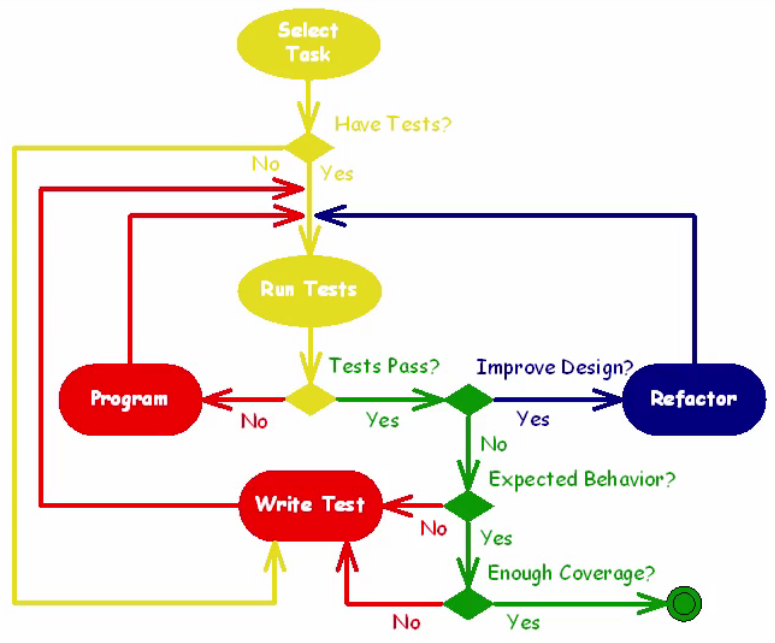
\includegraphics[width=0.8\linewidth]{img/tdd_cycle_detail}
	\caption{TDD Lifecycle in Depth}
	\label{fig:tddcycledetail}
\end{figure}

\section{Code Smells}
Ein Code Smell ist ein Hinweis auf ein schwerwiegenderes Problem (Design Flaws), dass besser behoben werden sollte. (If it stinks, change it) Wie Weinkenner, haben auch Programmierer ein eigenes Vocabular, um Smells genau zu beschreiben.

\subsection{Technical Dept}
Technical Dept ist eine Metapher für die möglichen Konsequenzen schlechter technischer Umsetzung von Software. Man versteht darunter den zusätzlichen Aufwand, den man für Änderungen und Erweiterungen an schlecht geschriebener Software einplanen muss. 
\begin{itemize}
	\item Nicht Aktualisieren von Softwaredokumentation
	\item Fehlende Versionierung, Backup, Build-Tools, CI
	\item Aufschieben und Verzicht von automatisierten Tests
	\item Missachtung von TODO und FIXME
	\item Codewiederholungen und andere Code Smells
	\item Missachtung von statischer Code Analyse
\end{itemize}

\subsection{Ursachen}
\begin{itemize}
	\item Fachlicher Drucker
	\item Ungenügende qualitätssichernde Prozesse
	\item Ungenügendes Wissen / Kommunikation
\end{itemize}

\subsection{Lost Intent}
Beim Lost Intent ist die Absicht nicht klar ersichtlich.
\begin{lstlisting}
// constructors
public Loan(commitment, riskRating, maturity);
public Loan(commitment, riskRating, maturity, expiry);
public Loan(commitment, outstanding, riskRating, maturity);
public Loan(capitalStrategy, commitment, riskRating, maturity, expiry);
public Loan(capitalStrategy, commitment, oustanding, riskRating, maturity, expiry);

// refactorings
private Loan(capitalStrategy, commitment, outstanding, riskRating, maturity, expiry);

public createTermLoan(commitment, riskRating, maturity, expiry);
public createTermLoan(commitment, outstanding, riskRating, maturity);
public createResolver(capitalStrategy, commitment, riskRating, maturity, expiry);
public createRCTL(capitalStrategy, commitment, oustanding, riskRating, maturity, expiry);
\end{lstlisting}

\subsection{Inefficient Name}
Unverständliche Namen erschweren die Arbeit des Programmierers, da es schwierig ist die Funktionlität bei schlecht gewählten Namen zu eraten. Möchte man die Performance eines Programmcodes verbessern, startet man oft an der Stelle die am meisten aufgerufen wird. Genau gleich sollte es mit der Performance des Programmierers sein. Programmierer verwenden einen grossen Teil ihrerer Zeit für das Lesen und Verstehen von Code. Damit wird die Performance des Programmierer verbessern können, müssen wir den Code lesbar schreiben. Gute Namen beantworten die Frage nach dem Warum sollte jemand diese Methode, Variable, Klasse verwenden.

\begin{lstlisting}
squareRootOfSumOfDimensionalDifferences -> distance
setBit7OnRegister3() -> turnOnLoopbackMode()
\end{lstlisting}

\paragraph{Gute Namen} sind simple, accurate, consistent.

\subsection{Duplicate Code}
Man unterscheidet zwischen zwei Varianten von Code Duplizierung:
\begin{description}
	\item[Blatant] Der genau gleiche Code kommt an mehreren Stellen vor
	\item[Subtle] Scheinbar unterschiedlicher Code führt die selbe Funktionalität aus (gleiches Boilerplate, einzelne unterschiedliche Methoden werden aufgerufen)
\end{description}

\section{Error Handling}

\subsection{Vermeidung}
Es gibt mehrere Möglichkeiten, Fehler zu vermeiden:
\begin{itemize}
	\item Testing / Simulation schreiben
	\item Statische Analyse
	\item Architektur (Review)
	\item Deliberate Programing
	\item Reviews
\end{itemize}

Werkzeuge zur Fehlerbehandlung sind:

\begin{itemize}
	\item Exceptions (machen alles einfacher)
	\item Assertions
	\item Logging
\end{itemize}

\subsection{Defensive Programmierung}

Defensive Programmierung beinhaltet eine systematische Fehlerprüfung von allen Inputs, sowie eine \textbf{systematische Fehlerbehandlung}. Defensive Programming macht nur in bestimmten Anwedungsbereichen Sinn, da es mit einem grösseren Aufwand verbunden ist.

Dies umfasst:
\begin{itemize}
	\item Behandeln und Filtern von Benutzereingaben. Anzeigen von Fehlermeldungen und Aktion unterbinden.
	\item Prüfen von allen Daten aus externen Quellen
	\item Prüfen von Routinen-Preconditions
	\item Ungültige Fälle systematisch abfangen (z.B. Exception werfen als default in switch-case $\rightarrow$ Nicht unterstützte Zustände systematisch abfangen. Somit werden Fehler durch spätere Erweiterungen besser erkannt)
\end{itemize}
	
\subsubsection{Fehler-Barrikaden}

Eine Fehler-Barrikade ist ein geschützter Rahmen mit sichergestellt validen Daten. So könnte man z.B eine Facade erstellen, die einen String auf seine Korrektheit überprüft und den String dann in ein URL Objekt packt, wobei die URL immutable sein sollte. Damit bleibt der String innerhalb der Barrikade konsistent.
\begin{itemize}
\item Barrikade im Programm gegen Fehler definieren
	\begin{itemize}
		\item Hinter den Barrikaden sind Daten gültig
		\item Daten bei Grenzübertritt überprüfen
	\end{itemize}
\item Barrikade auf Klassenniveau
	\begin{itemize}
		\item Public Methoden überprüfen Daten
			\begin{itemize}
			\item Per  Exception (externer Input)
			\end{itemize}
		\item Private Methoden gehen von gültigen Daten aus
			\begin{itemize}
				\item Per Asserts (interner Input)
			\end{itemize}
	\end{itemize}
\end{itemize}


\subsection{Fehlerhandling}

\paragraph{Konservative / Pessimistische Behandlung:}
\begin{itemize}
	\item Error handling prozedur
	\item Fehlermeldung anzeigen
	\item Shutdown
\end{itemize}

\paragraph{Optimistische Behandlung:}
\begin{itemize}
	\item Neutrales Resultat
	\item Nächstes plausibles Resultat
	\item Warnung in Stream loggen
	\item Optimistische Fehlerbehandlung kann in einem kritischen System gefährlich sein, wenn die getroffenen Annahmen/default Werte falsch gewählt wurden. Bei optimitischer Fehlerbehandlung sollte deshalb immer ein Log erstellt werden. 
\end{itemize}

\subsubsection{Korrektheit und Robustheit}
\begin{description}
	\item[Korrektheit] Niemals ein ungenaues Resultat liefern (Oft bei Sicherheistkritischen Systemen: z.B Bank Trading)
	\item[Robustheit] Die Software wenn möglich am Laufen zu halten. (Meist bei unkritischen Systemen: z.B Betriebsystem)
\end{description}

\subsubsection{Lokale vs. globale Behandlung}
\begin{itemize}
	\item Lokale fälle sind erwartete Fälle, die nicht höher relevant sind und lokal abschliessend entscheidbar sind. Checked Exceptions sollten lokal behandelt werden.
	\item Ansonsten sollte die Exception weitergegeben werden.
	\item Wichtig: Immer gültige Zwischenzustände mit \lstinline|finally| hinterlassen
	\item Eine Top-Level Behandlung soll alle Fälle abfangen, behandeln, protokollieren und dem Benutzer eine Meldung abgeben. Falls möglich kann das Programm darauf in einen konsistenten Zustand versetzt oder kontrolliert terminiert werden.
	\item Error Handling sollte auch getestet werden.
\end{itemize}

\subsubsection{Exceptions vs. Assertions}

\begin{itemize}
	\item Exceptions für produktive Fälle und sicherheitsrelevante Fehler.
	\item Assertions sind mehr für Debugging, Fehler welche nie auftreten sollten sowie Post/Preconditions. Sie sollten eher zwecks Dokumentation genutzt werden.
	\item Achtung: Assertions können Nebeneffekte haben, und können ein Programm in einem inkonsistenten Zustand belassen. z.B wenn der \lstinline|assert| etwas ausführt, bevor ein boolscher Wert zurückgegeben wird.
\end{itemize}


\subsection{Logging}
Logging dient der Postmortum-Analyse. Es empfiehlt sich ein Plan zu erstellen, wann und auf welchem Level geloggt wird.
\begin{itemize}
	\item Logging existiert zu diagnostischen Zwecken. Üblicherweise gibt es verschiedene Log-Levels.
	\item Für das Logging empfiehlt es sich, ein passendes Framework einzusetzen (z.B. log4j oder log4net)
\end{itemize}


\subsection{Policies}

\begin{description}
	\item[Error Handling Policy] \hfill \\
	Welche Eingaben und Interaktionen sind erlaubt und wie soll sich das System bei Fehleingaben verhalten?
	\item[Exceptions Policy] \hfill \\ Werden Exceptions benutzt und wie soll dies gemacht werden?
	\item[Assertion Policy] \hfill \\ Werden und für was werden Assertions benutzt und wann werden sie eingeschaltet?
	\item[Logging Policy] \hfill \\ Was und wie detailiert wird in das Log geschrieben? Welche Log Levels werden verwendet?
\end{description}


\section{Design by Contract}

\begin{itemize}
	\item Contracts (Verträge) legen Benefits (Rechte) und Obligations (Pflichten) zweier Parteien, meist Client und Supplier, fest.
	\item Design by Contract legt die Beziehung zwischen Komponenten fest.
	\item Erfunden wurde es mit dem Hoare Trippel: $\left\{P\right\} c \left\{Q\right\}$ (Precondition $P$, Programm $c$, Postcondition $Q$). 
	\item Bertrand Meyer entwickelte dieses Konzept zur Designmethode und Sprache Eiffel weiter.
\end{itemize}


\subsection{Preconditions, Postconditions, Class Invariants}

Für jede Methode gibt es:

\subsubsection{Preconditions}

Dies sind Bedingungen, welche vor dem Aufruf erfüllt sein müssen. Der Aufrufer ist für dessen Einhaltung verantwortlich.

\subsubsection{Postcondition}
Dies sind Bedingungen, welche nach dem Aufruf erfüllt sein müssen. Dafür ist die Implementation der Methode zuständig.

\paragraph{Bei Query-Only Methoden}, welche den internen Zustand nicht ändern, sind keine Postconditions auf interne Zustände möglich. Es gibt höchstens Postconditions für Rückgabewerte.


\subsubsection{Class Invariants}

Die Klasseninvarianten stellt für eine Klasse gewisse Garantien sicher, welche vor und nach dem Methodenaufruf gelten. Dafür ist die Implementation der Klasse verantwortlich.


\subsubsection{Eiffel: Beispiele}

\begin{lstlisting}[language=eiffel]
put (x: ELEMENT; key: STRING) is
-- Insert x so that it will be retrievable through key.
require
	count < capacity
	not key.empty
do
	-- ...Some insertion algorithm ...
ensure
	has (x)
	item (key) = x
	count = old count + 1
end
\end{lstlisting}

\begin{lstlisting}[language=eiffel]
class STACK
-- ...
invariant
	count_non_negative: 0 <= count
	count_bounded: count <= capacity
	consistent_with_array_size: capacity = representation lcapacity
	empty_if_no_elements: empty = (count = 0)
	item_at_top: (count > 0) implies
		(representationl item (count) = item)
end
\end{lstlisting}


\subsubsection{Einschränkungen}

Interne Konsistenzen wird nicht überprüft, es werden nur die Interfaces überprüft. 

\subsection{Gute Verträge, Anwendung in agilem Umfeld}

Ein Vorteil guter Verträge ist ein besseres Verständnis, wer wofür verantwortlich ist.
Preconditions: Client, Postconditions: Supplier


\subsection{Exceptions}

Exceptions werden unterschieden in normale  und exceptional Exceptions. Bei Exceptional können andere Postconditions greifen als bei Normalen.

\subsection{Vererbung}

Erbende Klassen müssen immer \emph{mindestens} die Conditions der Superklasse oder des Interfaces erfüllen. D.h. Preconditions dürfen gleich bleiben oder gelockert werden, Postconditions dürfen verschärft, aber nicht gelockert werden. Die Invariante darf gleich bleiben oder verschärft werden. (Liskov Substitution Prinzip oder Behavioural Subtyping $\rightarrow$ Subtyp muss mindestens den Vertrag der Basisklasse erfüllen.)

\subsection{TDD}

Contracts sind eine optimale Ergänzung zu Unit Tests bei der TDD-Entwicklung.

TDD Prinzipien für einen Clean Contract:
\begin{enumerate}
	\item Trenne Abfragen durch @Pure von Kommandos
	\item Trenne elementare Abfragen von abgeleiteten Abfragen
	\item Erstelle für jede abgeleitete Abfrage eine Nachbedingung
	\item Erstelle für jedes Kommando eine Nachbedingung
	\item Prüfe für jede Abfrage und jedes Kommando, ob eine Vorbedingung erforderich ist
	\item Formuliere Invariante, um unveränderliche Eigenschaften des Objekts beschreiben.
\end{enumerate}

DbC Konstrukte sind deklarativ, Unit Tests sind imperativ. DbC kann als Ergänzung zu Unit Tests angesehen werden. Unit Tests testen in der Regel auch Postconditions.

\subsection{Unterstützung von DbC in Programmiersprachen}

Es ist grundsätzlich empfehlenswert, in einer Sprache, welche keine Native Unterstützung für Contracts hat, ein passendes Framework zu verwenden.

\subsection{Java}

Z.B. mit icontract:

\begin{figure}[h]
	\centering
	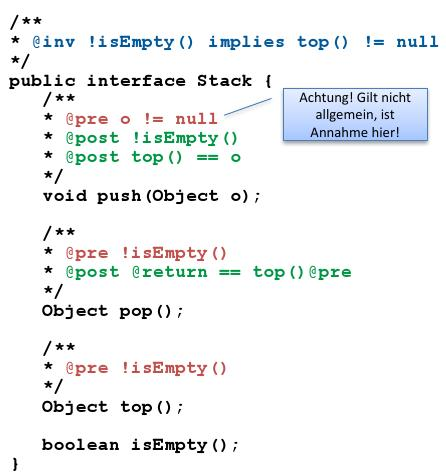
\includegraphics[width=0.7\linewidth]{img/contracts_java_icontract}
	\caption{Contract in Java mit icontract}
	\label{fig:contractsjavaicontract}
\end{figure}

\paragraph{Frameworks}: Contract4J, JML, Oval, Cofoja


\subsection{Concurrency}
Alle bisherigen Aussagen gelten nur wenn entweder die Programme sequentiell ausgeführt werden oder es sich um fully synchronized objects handelt.

\section{Code Smells}

Die sechs häufigsten Code Smells sind:

\begin{itemize}
	\item Duplicated Code
	\item Long Method
	\item Large Class
	\item Conditional Complexity
	\item Comment Smell
	\item Switch/Case (insbesonders wenn instanceOf() im Spiel ist)
\end{itemize}


\subsection{Prüfungsrelevanz}

In der folgenden Liste sollten Sie an einer Prüfung:
\begin{itemize}
	\item Einen Smell erkennen, wenn er als Code daherkommt
	\item Wenn der Smell-Name gegeben ist, beschreiben was das das Problem mit dem Smell ist
	\item Wenn der Name vorgegeben ist, ein gutes Beispiel hinschreiben können (Code-Fragment skizzieren)
\end{itemize}

Liste der Smells, die Sie kennen sollten:

\begin{multicols}{2}
	\begin{itemize}
		\item Speculative Generality
		\item Comment
		\item Long Method
		\item Long ParameterList
		\item Magic Numbers
		\item Duplicated Code
		\item Large Class
		\item Conditional Complexity
		\item Switch/Case (ibs. wenn instanceOf() im Spiel ist)
		\item Primitive Obsession
		\item Oddball Solution
		\item Refused Bequest
		\item Inapporpriate Intimacy
		\item Feature Envy
		\item Lazy Class
		\item Middle Man
		\item Shotgun Surgery/Solution Sprawl
	\end{itemize}
\end{multicols}

\section{Refactoring}
Unter Refactoring versteht man eine Änderung der interenen Struktur von Software, sodass diese einfacher zu verstehen und günstiger abzuändern ist, jedoch ohne dass das Verhalten der Software verändert wird. Typischerweise wird bem Refactoring folgende Dinge unternommen:
\begin{itemize}
	\item Removing duplicated or dead code
	\item Simplifying complex code
	\item Clarifying unclear code
\end{itemize}

\subsection{Pattern}
Die sechs häufigsten refactoring patterns sind:

\begin{itemize}
	\item Extract Method
	\item Rename
	\item Move Method (inklusive pull up/push down)
	\item Change Method Signature
	\item Replace Inheritance with Delegation
	\item Replace Magic Number with Symbolic Constant
\end{itemize}

\subsection{Refactor Zyklus}
Es lohnt sich ein Refactoring in vielen kleinen Schritten (Baby Steps) durchzuführen.
\begin{enumerate}
	\item Verify that all automated tests (microtests) pass
	\item Decide what code to change
	\item Implement one or more refactorings carefully
	\item Run the microtests whenever you wish to confirm that changes have not altered system behavior
	\item Repeat until the refactoring is complete or revert to an earlier state
\end{enumerate}

\begin{figure}[h]
	\centering
	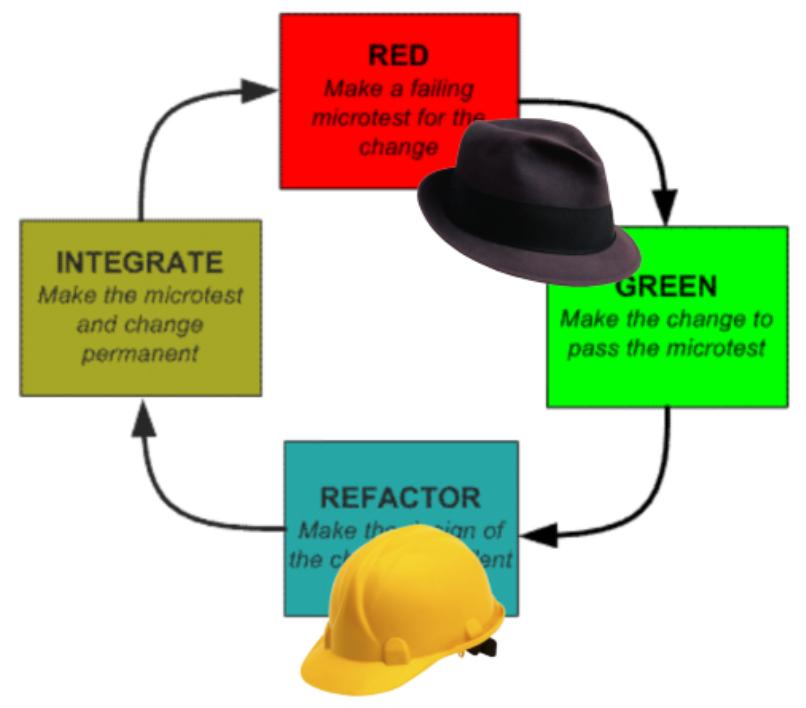
\includegraphics[width=0.6\linewidth]{img/refactoring_cycle}
	\caption{Refactoring Cycle}
	\label{fig:refactoringcycle}
\end{figure}

\subsection{Prüfungsrelevanz}

Die folgende Liste definiert, welche Refactorings Sie gut kennen sollten, insbesonders:

\begin{enumerate}
	\item erkennen und benennen können, wenn die Refactorings als Vorher/Nachher-Bilder (UML) oder Code daherkommen
	\item wenn Refactoring-Name erwähnt, beschreiben, was passiert
	\item wissen, welchen Smell das Refactoring behebt, und wann Sie es anwenden
	\item Antworten können: gegeben Smell X, welches Refactoring ist hier zielführend? (mehrere möglich, nur 1 nötig für korrekte Antwort)
\end{enumerate}

Liste der Refactorings:

\begin{multicols}{2}
	\begin{itemize}
		\item Extract Method, Inline Method
		\item Extract Variable, Inline Temp
		\item Replace Temp with Query
		\item Rename Method/field/parameter
		\item Move Method (inkl. pull up/push down)
		\item Move Field (inkl. pull up/push down)
		\item Change Value to Reference, Change Reference to Value
		\item Replace Magic Number with Symbolic Constant
		\item Change Method Signature
		\item Encapsulate Field
		\item Replace Type Code with Class/Subclass
		\item Replace Type Code with State/-Strategy
		\item Decompose Conditional
		\item Replace Nested Conditional with Guard Clauses
		\item Introduce Null Object
		\item Replace Constructor with Factory Method
		\item Replace Exception with Test
		\item Extract Subclass/Superclass
		\item Extract Interface
		\item Collapse Hierarchy
		\item Replace Inheritance with Delegation
		\item Oddball Solution: Substitute Algorithm [Fowler], Unify Interfaces with Adapter (GOF)
	\end{itemize}
\end{multicols}

\subsubsection{Nutzen}
\begin{itemize}
	\item Pull Up Method $\rightarrow$ Duplication Free
	\item Pull Down Method $\rightarrow$ Highly Cohesive
	\item Rename Method $\rightarrow$ Clarity
	\item Replace Inheritance With Delegation $\rightarrow$ Highly Cohesive
	\item Split Temporary Variable $\rightarrow$ Clarity
\end{itemize}

\subsection{Eclipse Integration}
Alle grösseren IDE bieten heutzutage automatische Refactoring Funktionalität an.

\begin{itemize}
	\item Move..
	\item Change Method Signature
	\item Extract Interface 
	\item Extract Superclass
	\item Pull Up
	\item Push Down
	\item User Supertype where possible
	\item Introduce Parameter Object
	\item User Supertype where possible
	\item Infer Generic Type Arguments
\end{itemize}

\section{Aufteilung Projekte / Story splitting}

Grosse Projekte schlagen oft fehl, darum möglichst nie Projekte mit > 9 Monate, > 1 Million Budget oder Team > 10 Personen! Falls Projekte grösser werden, müssen sie aufgesplitted werden.

\subsection{Aufteilung im Grossen}
\subsubsection{Aufteilungs- und Priorisierungskriterien}

\begin{itemize}
	\item Nach Kundendomänen
	\item Nach Geschäftsprozessen (ungefähr nach User Cases)
	\item Nach Benutzerrollen (z.B. Alle Endbenutzerprozesse, Administratorfunktionen)
	\item In Kern Funktionen, Wichtige Funktionen, 08/15 Funktionen, CRUD
	\item Nach Bereiche im Domain-Model
	\item Geografisch (z.B. zuerst Kanton GR, dann erst ZH)
\end{itemize}

\subsection{Aufteilung im Kleinen}
Zuerst minimale Grundfunktionen bauen, später Features inkrementell nachliefern. Man spricht von dem Minimum Viable Product (MVP) $\rightarrow$ A product with just enough features to gather validated learning about the product. Der Kostensprung von der Basis Version zum Voll-Ausbau darf nicht vernachlässigt werden. (1:10)

\subsection{Arbeitspakete / User Stories}
User Stories sind umsetzungsorientiert und auf den Arbeitsfluss/Sprintgrösse angepasst. (Im Gegensatz zu den Use Cases, diese sind kundenorientiert). 

\begin{description}
	\item[Durchschnitt:] was 1 Person in 1/4 eines Sprints schafft
	\item[Maximum:] was 1 Person in 50-70\% eines Sprints schafft
\end{description}


\subsection{Story Mapping}
Zusammenfassen mehrerer User Stories zu einer grösseren Einheit (meist Epics), für mehr Übersicht. 


\begin{figure}[h!]
	\centering
	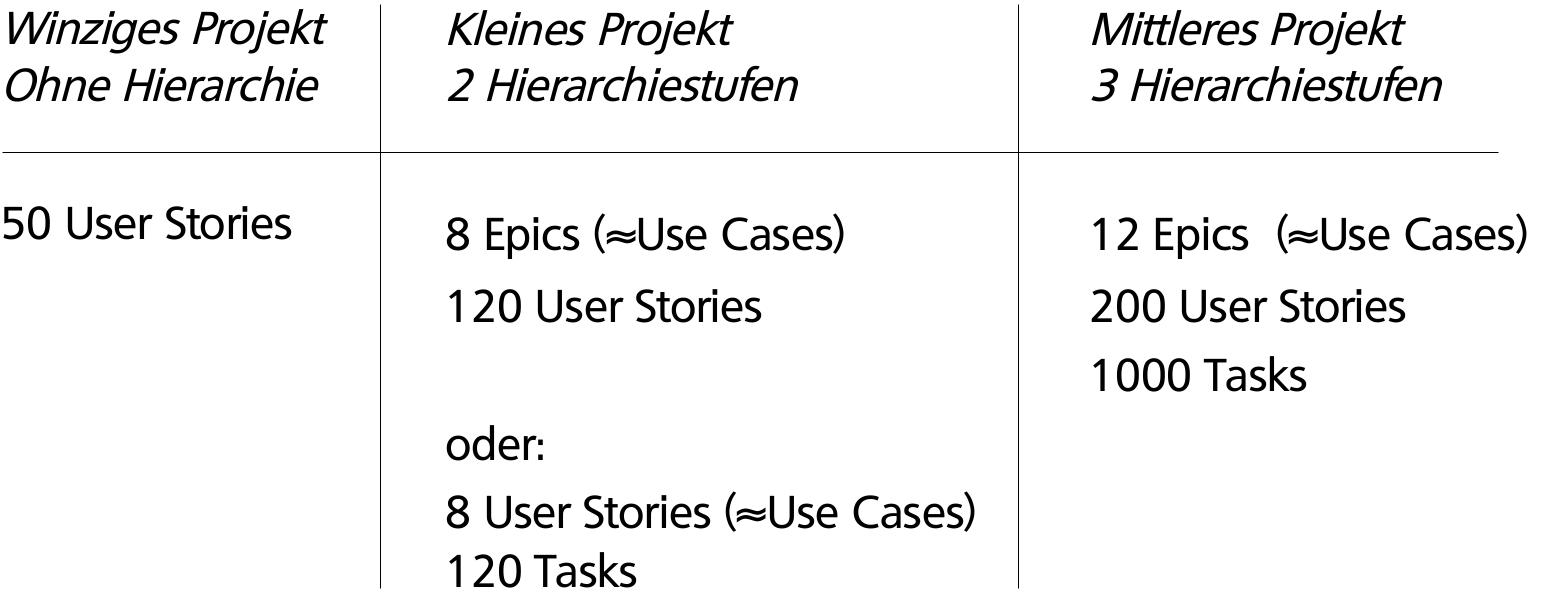
\includegraphics[width=0.6\linewidth]{img/projektuebersicht}
	\caption{Projektübersicht / Aufteilung Projekte}
	\label{fig:projektuebersicht}
\end{figure}



\section{Testing: Unit Tests and More}

\begin{figure}[h!]
	\centering
	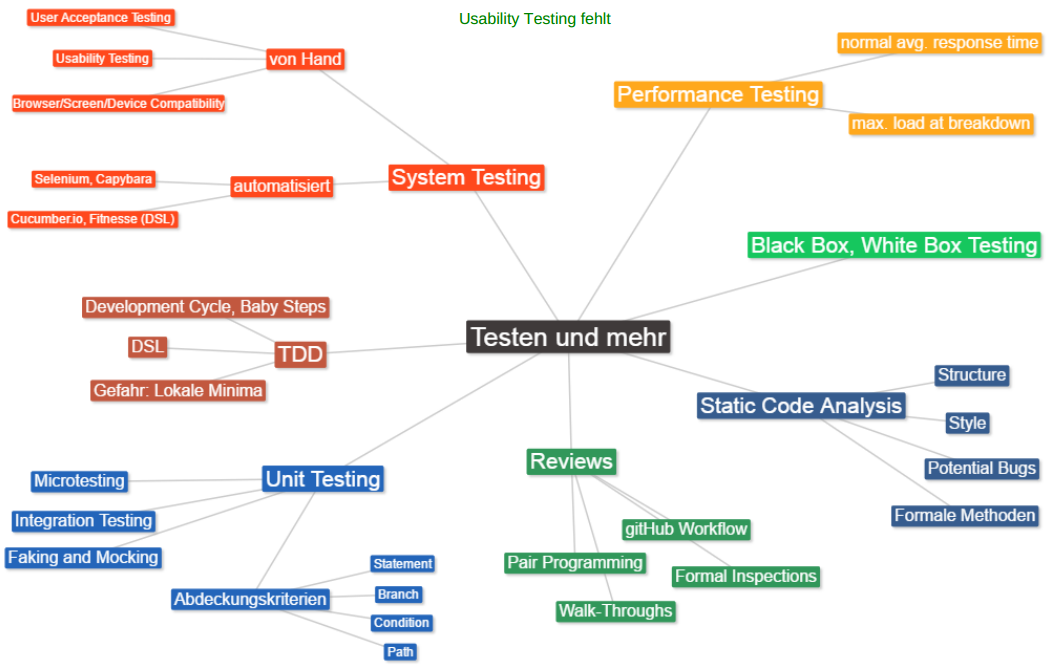
\includegraphics[width=0.7\linewidth]{img/testing_overview}
	\caption{Übersicht von Tests}
	\label{fig:testingoverview}
\end{figure}


\subsection{Unit Tests / Microtests}

Isoliertes Testen einer Klasse bzw. meist einzelner Methoden. Sollte schnell gehen (wichtig für CI). Wird oft in Kombination mit Fakes \& Mocks eingesetzt.

\paragraph{Nachteile} von Unittests sind oft die fehlende Aussagekraft, durch welche sich so mancher in falsche Sicherheit wiegen lässt. Sie funktioneren gut auf tiefen Layers sowie in Libraries, aber nur mit Einschränkungen auf höheren Layers.

\subsubsection{Faking \& Mocking}
\begin{description}
	\item[Fakes,] manchmal Stubs genannt sind ein simpler Ersatz, meist mit fixen Daten.
	\item[Mocks] geben intelligente Rückgabewerte und schaut/kontrolliert, ob und die Funktionen aufgerufen wurden.
\end{description}

\subsubsection{Fallbeispiele Externe Dienste:}
\begin{description}
	\item[FTP-Server] FTP-Server: Nicht wegmocken, lieber lokalen Testserver aufsetzten (Docker o.ä.)
	\item[Börsenkurse] Wegmocken, da auch (noch) nicht reale Szenarien getestet werden sollen.
\end{description}

\subsubsection{Coverage}
Es gibt verschiedene Arten von Coverage:

\begin{description}
	\item[Anweisungsabdeckung (Statement Coverage)] ist die Meistverwendete Variante, sie zählt Zeilen, welche durch Tests abgedeckt sind.
	\item[Zweigabdeckung (Branch Coverage)]  bedeutet,  jeder mögliche Programmzweig (if/else, switch etc.) wird gezählt.
	\item[Bedingungsabdeckung (Decision Coverage)]  Das Verhältnis von ausgewerteten atomaren Werten (Term, Bedingung, ...) innerhalb von Ausdrücken zu allen vorhandenen atomaren Werten in einem Modul.
	\item[Pfadabdeckung (Path Coverage)]  Das Verhältnis der getesteten Pfade (Wege im Kontrollflussgraph), zu allen möglichen Pfaden in einem Modul. Die Pfadabdeckung ist kaum realistisch, da alle möglichen Kombinationen von Zweigen getested werden müsten.
\end{description}

Eine Coverage von 100\% ist so gut wie ausgeschlossen, da Spezialfälle wie ungewöhnliche Exceptions aufgrund von Nebeneffekten nur schwer simuliert werden können. Der Coverage-Prozent Indikator ist daher eigentlich nur als Negativaussage nutzbar (z.B. 20\% Coverage ist zu wenig).

\begin{remember}{Testabdeckung}{}
Eine hohe Testabdeckung ist eine notwendige aber nicht hinreichende Bedingung. Wichtig ist die Qualität und nicht die Abdeckung. Integrationstests sind wertvoller wie Microtests.
\end{remember}

\subsection{Integration Tests}

Integration Tests sind eigentlich Unit Tests auf höheren Etagen. Sie testen das System als Black Box, und sind daher langlebiger als Microtests. Drittsysteme werden manchmal gefakted oder weggemockt, oft aber auch direkt angesprochen (z.B. lokaler Datenbankserver). Integrationstests entdecken mehr Fehler, weils sie realistischere Szenarious testen. 

Ein grosser Nachteil von Integration tests ist, dass diese oft sehr langsam sind, und sich daher nicht für CI eigenen.


\subsection{Konsistenz-Tests für Datenbanken}

Konsistenz-Tests für Datenbanken sind SQL Statements, welche wie Unittests die Konsistenz der Datenbank prüfen können. z.B. Gibt es Kunden, bei denen kein richtiger Namen eingetragen ist?


\subsection{Build Server}

Ein Build Server hat üblicherweise folgende Aufgaben:
\begin{itemize}
	\item fetch from git
	\item compile, build EXE
	\item run Unit Tests
	\item run metrics
	\item run findbugs, checkstyle
	\item log everything
	\item dashboard (z.B. sonarQube)
\end{itemize}

Da es bei vielen Entwicklern häufig zu Build fehlern kommt, ist es ratsam, grosse Projekte im CI zu unterteilen.


\subsubsection{Build Strategien}
\begin{description}
	\item[Daily Build, Nightly Build] \hfill \\ Einmal alle 24 Stunden (weil der Build und die Tests sehr lange dauern, z.B. 6 Stunden)
	\item[Daily Build] \hfill \\ Alle drei Stunden (weil der Build jedesmal ca. eine Stunde dauert)
	\item[Continuous Integration] \hfill \\ Jedesmal, wenn ein commit auf den Haupt-Zweig gemacht wird (weil ein Build weniger als 10 Minuten dauert)
	\item[CI mixed] \hfill \\ Tagsüber Continuous Integration mit allen schnellen/billigen Tests, nachts (oder alle drei Stunden) die vollen Tests
\end{description}

\subsubsection{Deployment systeme}

Oft gibt es folgende deployment (meist teilautomatisierte) Systeme:
\begin{description}
	\item[Development] \hfill \\ Entwicklersystem (relativ stabil für alle Entwickler), Daily Build / CI Machine
	\item[Test] \hfill \\ Stabile Test-Umgebung für die Entwickler Alle automatisierten Tests Erste Performance-Tests
	\item[Acceptance / Staging] ($\approx$ Staging): \hfill \\ Manuelles Testen durch Kunde und externe Tester; HW \& Testdaten möglichst gleich wie PROD (ausser bei Deployment-Änderungen); hier auch Performance-Tests
	\item[Productive] \hfill \\ Produktiv-Umgebung, muss stabil sein, keine Experimente! Neue Releases nur alle paar Monate.
\end{description}

Testdaten werden üblicherweise vom Productive richtung Development-System übernommen und z.T. anonymisiert.

Das Testsystem sollte etwa täglich, Acceptancesystem bei Sprint Ende und das Produktivsystem etwa alle zwei Monate propagiert werden.

\section{Aufwandschätzung}

Rund 70\% der Informatik Projekte sind nicht erfolgreich oder über dem Budget. Dabei kommt es öfter zu ''Scope Creep'', d.h., der Umfang des Projekts wurden laufend erhöht und geändert.

\begin{remember}{Faustregel}{}
Grosse Projekte schlagen oft fehl, darum möglichst nie Projekte mit > 9 Monate, > 1 Million Budget oder Team > 10 Personen!
\end{remember}

Die Kommunikation zwischen Teammitglieder verhält sich mit $\frac{n \cdot (n - 1)}{2} \rightarrow \mathcal{O}(n^2)$, was einer der grössten Einflussfaktoren eines Projektes ist. Dazu kommen weitere nicht-lineare Faktoren: 

\begin{multicols}{2}
\begin{itemize}
	\item Communication 
	\item Planning
	\item Management
	\item Requirements development
	\item System functional design
	\item Interface design and specification
	\item Architecture
	\item Integration
	\item Defect removal
	\item System testing
	\item Document production
	\item Unterschiedliche Auffassung in der Vision
	\item Unterschiedliches technisches Verständnis
	\item Unterschiedliche Muttersprache
\end{itemize}
\end{multicols}



\subsection{Warum gibt es Fehlschätzungen}

\begin{itemize}
	\item Politische Vorgaben dominieren, nicht realistische
	\item Zuviel Optimismus
	\item Fehlende Sorgfalt, mangelnde Qualität (quick \& dirty stays)
	\item komplexität und unerwartete Nebeneffekte zerstören die Pläne
	\item \textbf{Fehlende Erfahrung/Übung}
\end{itemize}

\subsection{Einflussfaktoren}

Nach ISBSG.org:

\begin{enumerate}
	\item Project size
	\item Size of customer base (how many installations)
	\item Stability of requirements
	\item Cooperation with customer (customer in team)
	\item Team fitness/quality
	\item Complexity of system (real-time, distributed, multi-platform,edge of technology)
	\item Security and safety requirements (banking, medical)
\end{enumerate}

\subsection{Vorgehensweisen}

\subsubsection{Top-Down}

Zuerst das Gesamte, dann Teilbereiche schätzen. Wird meistens zu Begin der Elaboration-Phase gemacht.

\paragraph{COCOM-Schätzung}
%TODO ist das relevant?


\subsection{Bottom-Up}

Bei vorliegen aller Requirements, Arbeitspakete sowie einem Entwurf; die einzelnen Elemente werden geschätzt in der Grössenordnung von 0.5 bis 3 Tagen.

Wird meistens gegen das Ende der Elaboration-Phase gemacht.


\subsection{Arbeitsfortschritt}

Meistens nimmt der Arbeitsfortschritt keine lineare Form, sondern eher die Form eines Sigmoids an. Dies hat folgende Gründe:
\begin{itemize}
	\item Schwieriges wird (unbewusst) hinausgeschoben, bzw. nicht genau genug abgeschätzt. 
	\item Umgesetze Funktionen funktionieren zwar, verursachen aber an anderen Orten Probleme. 
	\item Kunde sieht SW funktionieren, jetzt kommen Korrekturen und Wünsche. 
	\item Refactoring verbessert den Code ohne dass mehr Funktionalität sichtbar ist. Der Kunde sieht den Fortschritt nicht
	\item Verbesserungen von Robustheit oder Security kosten viel Arbeit, führen aber nicht zu sichtbarer Funktionalität.
\end{itemize}

\begin{figure}[h]
	\centering
	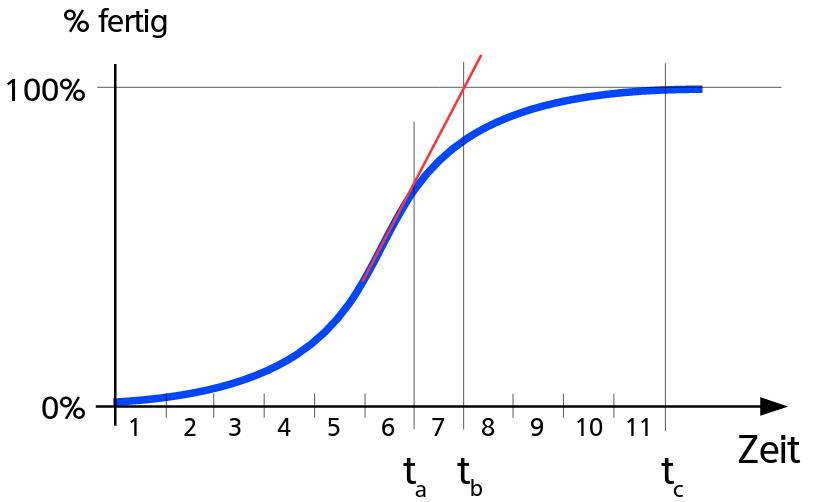
\includegraphics[width=0.8\linewidth]{img/arbeitsfortschritt_sigmoid}
	\caption{Arbeitsfortschritt (Sigmoid)}
	\label{fig:arbeitsfortschrittsigmoid}
\end{figure}

\begin{itemize}
	\item $t_a$: Alle läuft gut, das Team ist optimistisch
	\item $t_b$: Der Projektabschluss Zeitpunkt wird von dem optimistischen Team extrapoliert. 
	\item $t_c$: Tatsächlich get das Projekt aber noch 5 mal so lang, denn die letzten Reste aufzuräumen kostet überproportional viel (80/20 Regel).
\end{itemize}

Dauert ein Projekt mit 10 Entwickler 2 Jahre, macht es keinen Sinn, das Projekt in einem Jahr mit doppelt so vielen Entwickler umzusetzen. Der Aufwand und somit die Kosten steigen stark an. 

\subsubsection{LOC pro Monat}

Gemessen am gesamten Team inkl. Administration und ohne Tests.

\begin{description}
	\item[80-150 LOC] bei schwierigen Echtzeit-Projekten (Zahl v. IBM, Space Shuttle)
	\item[300-500 LOC] im Schnitt mit einem guten, nicht zu grossen Team
	\item[bis ca. 1000 LOC] nur mit kleinen Spitzenteams
	\item[über 1500 LOC] ist unglaubwürdig (Pfusch, viel Copy/Paste, generiert)
\end{description}


\section{Software-Metriken}

\begin{itemize}
	\item Software-Metriken sind z.B. beim Einstieg in ein bestehendes, fremdes Projekt nützlich.
	\item Metriken sind immer Interpretationssache: Es ist schwierig, vernünftige harte Grenzen festzulegen.
	\item Entwickler sollten allerdings nicht nach Metriken belohnt werden: Kann unerwartete Nebeneffekte haben!
	\item Metriken die im Buildprozess integriert sind, geben nützliche Hinweise für ein allfälliges Refactoring.
\end{itemize}



\subsection{Kennmerkmale}

Es wird unterschieden in Produktmetriken (Kennzahlen der Software, Zyklomatische Komplexität) und Projektmetriken (Issues, Number of Commits, etc.). Der Fokus liegt in erster Linie auf Produktmetriken.

\begin{itemize}
	\item Suche nach *.* => was liegt überhaupt vor? welche Sprachen?
	\item Dokumentation lesen (und verifizieren ?=? tatsächliche Architektur)
	\item Eingesetzte Tools? (CVS, findbugs/checkstyle/ReSharper, cobertura...)
	\item Eingesetzte Libraries, Frameworks (zu wenig? veraltet?)
	\item Unit Tests? (genügende Abdeckung, sinnvolle Tests?)
	\item (Un)aufgeräumte Baustelle? (uneinheitlich, TODOs, dead code, ...)
	\item Welche Dateien werden am häufigsten ein- und ausgecheckt?
	\item Grösste Klassen finden (countlines, notfalls Dateigrösse in KB)
	\item Komplexität ermitteln (metrics, notfalls Suche nach '\&\&')
	\item Lesbarkeit?
	\item Erweiterbarkeit?
	\item Sicherheit, Robustheit, ...?
\end{itemize}

%TODO: Slides H. Rudin, FS15-SE2-09-Metrics.pdf

\subsection{Die Zyklomatische Zahl (McCabe Metrik)}

Misst Komplexität der logischen Struktur auf Basis des Kontrollflussgraph G eines Programmes.

Die Zyklomatische Zahl kann mit folgender Formel berechnet werden:

\[
	V(G) = e - n + 2p
\]

wobei

\begin{itemize}[label=""]
	\item[$e$] Anzahl Kanten (edges)
	\item[$n$] Anzahl Knoten (nodes)
	\item[$p$] Anzahl Komponenten (unabhängige Teil-Graphen]
\end{itemize}


Für eine einzelne Methode kann auch die vereinfachte Form verwendet werden: 
\[V(G) = \text{ Anzahl Verzweigungen (while, if, case) } + 1\]


\begin{remember}{Interpretation}{}
Ist die zyklomatische Zahl V(G) einer Funktion/Methode > 10, müss geprüft werden, ob sie eventuell zu vereinfachen ist.
\end{remember}


\subsection{Lack of Cohesion of Methods (LCOM*)}
* Variante nach [Henderson96]

\[
LCOM* = ( m - Mittelwert (m(A)) ) / ( m – 1)
\]


\begin{itemize}[label=""]
	\item[$m$] Anzahl Methoden
	\item[$m(A)$] Anzahl Methoden, die auf ein Attribut zugreifen
\end{itemize}

\paragraph{Interpretation:} LCOM* = 1 bedeutet schlechte Kohäsion, LCOM* = 0 bedeutet maximale Kohäsion


\subsection{Afferent und Efferent Coupling}
\begin{description}
	\item[Afferent Coupling] Eingehende Kopplung: Wie viele Klassen sind von mir abhängig? 
	\item[Effferent Coupling] Ausgehende Kopplung: Von wie vielen Klassen bin ich abhängig?
\end{description}

\subsection{Instability}

\[
	I = \frac{C_e}{C_a + C_e}
\]

\begin{description}
	\item[$C_a$] Afferent Coupling: Anzahl Klassen in einem Package, welche von Klassen innerhalb des Packages abhängen
	\item[$C_e$] Efferent Coupling: Anzahl Klassen eines Packages, welche von Klassen ausserhalb des Packages abhängen
\end{description}

\paragraph{Interpretation:} Umso kleiner $I$ ist, umso ''stabiler'' ist der Code (d.h., er hat wenig externe Abhängigkeiten). Stabile Klassen sind oft weit unten, da sie von vielen anderen Klassen verwendet werden. (I=0)

\subsection{Abstractness}
\[
A = \text{Number of abstract classes}
\]


\subsubsection{Normalized Distance from Main Sequence}

\[
	D_n = \left| A + I - 1 \right|
\]

\begin{description}
	\item[$I$] Instabilität (0-1)
	\item[$A$] Anzahl (abstrakter und normaler) Klassen eine Packages (0-1)
\end{description}

\paragraph{Interpretation:} $D_n$ sollte möglichst gering sein bei guten Package Design.

\paragraph{Zonen}
\begin{description}
	\item[Zone of Uselessness] In dieser Zone gibt es viele abstrakte Klassen, die nur von wenigen anderen Klassne gebraucht werden.
	\item[Zone of Pain] In dieser Zone gibt es viele konkrete KLassen mit vielen Abhängikeiten.
\end{description}

\begin{figure}[h!]
	\centering
	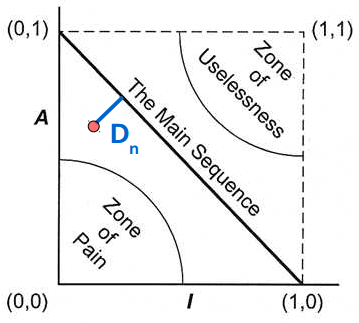
\includegraphics[width=0.5\linewidth]{img/abstractness_intability}
	\caption{Zone of Exclusions}
	\label{fig:abstractnessintability}
\end{figure}



\subsection{Tooling}
Für Software Metriken gibt es viele nützliche Tools in Java.

\subsubsection{Codeanalyse}

Codeanalysen helfen, die Codequalität in Projekten zu erhöhen.

Für die Visualisierung und Bearbeitung der nachfolgenden Metriken eignet sich SonarQube.

\paragraph{Für Java:}
\begin{description}
	\item[Structure101] Visualisiert Abhängikeiten von Code bzw. verschiedene Strukturelemente
	\item[Checkstyle (Java)] Prüft Quellcode nach Konventionen und einfachen Metriken
	\item[findbugs (Java)] Analysiert Bytecode nach logischen Fehlern
\end{description}

\paragraph{Für .NET:} NDepend, FXCop, ReSharper

\subsection{Zusammenfassung Metriken}

\begin{itemize}
	\item Oft: je grösser ein Projekt, desto mehr Fehler sind vorhanden.
	\item Metriken können schnell die neuralgischen Punkte aufzeigen. (keine Steigerung der Qualität)
	\item Metriken können zeigen, ob die Verbesserungen in die richtige Richtung gehen.
	\item Richtig gute Software-Qualitätsmetriken gibt es nicht; Abhilfe: Reviews.
	\item Metriken sind Interpretationssache (also Erfahrungssache und Sache von Spezialisten, daher auch nichts für Manager).
	\item Achtung: Manager lieben KPIs (Key Performance Indicators) und hätten gerne SW-Metriken dazu. Fast nie eine gute Idee.
	\item Metriken \& Belohnung = Desaster.
\end{itemize}


\section{Code Reviews}

Reviews sind eine sehr kosteneffiziente Art, Fehler zu entdecken. Zudem wird das Team insgesamt  besser und es gibt einen Know-How transfer.

Es gibt verschiedene Formalitätsgrade von Reviews:
\begin{itemize}
	\item[formlos:] Pair Programming
	\item Github Pull Requests
	\item Gruppen-Reviews
	\item[formal:] Formal Inspection (IBM)
\end{itemize}

\subsection{Gruppen-Reviews}

Meist mehrere Entwickler mit definierten Rollen (moderator, author/presenter, peer, note taker), welche in einer begrenzter Zeit (meist 2-4h) Code anschauen. Dabei wird ein Protokoll geschrieben.

Code Reviews sollten möglichst Zeitnah gemacht werden, da die Behebung mit der Zeit teurer wird. Dies gilt speziell für Regulierte Umgebungen.

\begin{enumerate}
	\item Stück Code oder Dokumentation auswählen (ca. 500 LOC pro 2h)
	\item Personen auswählen (peers) und Rollen verteilen (~3-5)
	\item Termin finden und Personen Einladen. Links zu Requirements, Architecture Document und Code anhängen.
	\item Personen sollten sich die Dokumente im Voraus kurz anschauen, statische Code Tests (\ref{sec:code-analysis-tools})
	\item Review durchführen \begin{itemize}
		\item Code walk-trough, geführt vom Autor
		\item Es sollte jeder in der Gruppe mal als Author im Review an die Reihe kommen.
		\item Kommentare der Reviewer im Protokoll notieren
		\item Erstes Ziel ist das finden von Fehlern.
		\item abschliessen der Bewertung mit \emph{Gut}, \emph{OK mit Nacharbeiten} oder \emph{nicht OK}
	\end{itemize}
	\item Nacharbeiten begleiten und abschliessen. Protokoll ablegen.
\end{enumerate}

\subsubsection{Wichtigste Fragen beim Code-Review}

\begin{itemize}
	\item Verständlichkeit (Warnsignal, wenn nicht alle den Code verstehen)
	\item Namenswahl (Methoden, Variablen, packages; das kann kein Tool)
	\item ''Code Smells'' (die üblichen Verdächtigen)
	\item Übereinstimmung mit Architektur-Ideen und Diagrammen
\end{itemize}

\subsubsection{Format des Protokolls}

\begin{itemize}
	\item Teilnehmende und deren Rollen, Zeit, Ort
	\item Identifikation des Code-Stücks und der relevanten Unterlagen
	\item Tabelle mit den offenen Punkten: ID, Beschreibung, Schweregrad, Datum \& Kürzel wenn behoben, Req.Ref. Bem.
	\item Aufgabenverteilung: Wer macht was bis wann (am besten gleich Issues erstellen)
	\item Verdikt („akzeptiert/akzeptiert mit Nacharbeiten/zurückgewiesen“
\end{itemize}

\subsubsection{Nacharbeiten}

Für jeden gefundenen Fehler:
\begin{itemize}
	\item mindestens einen Unit Test schreiben, der den Fehler provoziert
	\item Fehler beheben (und/oder refactoring) und dokumentieren
	\item Unit Test muss jetzt OK sein
\end{itemize}

\subsection{Code Analysis Tools}\label{sec:code-analysis-tools}

Code Metriken sind eine gute Unterstützung beim Code Review. Mit Tools können folgende Teilgebiete abgedeckt werden:
\begin{itemize}
	\item Code Metriken
	\item Überprüfung des Programmier-Stils
	\item Prüfung auf Anomalien und mögliche Fehler
	\item Auswertung der Testabdeckung
\end{itemize}

(metrics, checkstyle, ESLint, ReSharper, findbugs, EMMA, structure101 etc.)

Diese Tools sollten bei jedem Build sowie auf der Entwickler-Maschine laufen.

\subsection{Requirements Reviews}

Requirements Reviews helfen, von wolkigen Kundenwünschen zu formalen Requirements Specs zu kommen.

\subsection{Architektur-Reviews}

\begin{itemize}
	\item Nicht funktionale Anforderungen (u.a. Performance, Security)
	\item Kern-Charakteristiken des Systems
	\item Architektur-Dokumentation stimmt mit Implementation überein
	\item Szenarien durchspielen (z.B. ATAM Szenarien)
\end{itemize}


\section{Performance Messungen}

Voreilige Optimierungen für die Performance sind kontraproduktiv. Immer zuerst fragen: haben wir ein Problem?

Ein häufiger Fehler ist eine voreilige Parallelisierung.

Faustregel:
\begin{enumerate}
	\item Get it to run
	\item Get it right
	\item Make it fast
\end{enumerate}


\subsection{Java Profiling}

Tools:
\begin{itemize}
	\item NetBeans
	\item JProfiler
	\item AppDynamics
	\item NewRelic
\end{itemize}

\subsection{Last-Messungen (Black Box)}

Wann geht der Server in die Knie?

\subsubsection{Tools}
\begin{itemize}
	\item gatling.io, JMeter
\end{itemize}


\subsection{Performance-Messungen}

Sind die typischen Antwortzeiten immer noch etwas gleich?

\subsubsection{Tools}

\begin{itemize}
	\item Selenium (evtl. JMeter/gatling, diese können aber kein JS)
	\item Headless Browser
	\item Endlos viele Cloud Dienste
\end{itemize}

\subsubsection{Probleme mit Testdaten}

Mit testprozeduren gibt es ein Problem: Sie widerspiegeln oft nicht das Verhalten von Benutzern. Dies hat speziell Einfluss auf Caching und Memory Paging bei Datenbanken.

\subsection{Dashboards}

Dashbords helfen, einen schnellen Überblick über einen aktuellen Projektstand zu erhalten. Zielgruppe kann Business (z.B. Umsatzzahlen, Marketing-Effekt), Application (z.B. sizes Grösse von Tabellen), Server Infrastruktur

\subsubsection{Tools}

\begin{itemize}
	\item Grafana / Graphite
	\item Diverse Monitoring Lösungen
\end{itemize}


\section{Usability Testing}

\subsection{Zutaten}

\begin{itemize}
	\item Die neue, zu testende Software
	\item Mehrere nicht vorbelastete Nutzer (User)
	\item Ein Usability Lab
	\item Eine(n) Moderator(in) (facilitator, assistant)
	\item Mehrere Szenarien zum Testen (Use Cases)
\end{itemize}

\subsection{Durchführen}


Etwa in der Mitte des Projektes mit mindestens 3 geeigneten/normalen Testusern

\begin{enumerate}
	\item Kurze Einführung \begin{itemize}
		\item ''Helfen Sie uns'' ''Denken Sie laut'' '' Sie können nichts falsch machen'' ''Die Software wird getestet, nicht Sie''
	\end{itemize}
	\item Proband wird in ein Szenario eingeleitet
	\item Der Benutzer probiert ohne Hilfe, das Szenario zu ''lösen''. \begin{itemize}
		\item Der Beobachter macht Notizen, aber greift nicht ein
	\end{itemize}
	\item Erkenntnisse werden niedergeschrieben
	\item Bedanken beim Benutzer für die Wertvolle Hilfe
\end{enumerate}

\section{Architektur}

Architektur ist die Summe der Design-Entscheide, die von grosser Tragweite sind, und die länger leben.

Architektur ist die Aufteilung im Grossen.

IEEE STD 1472 Definition: ''An architecture is the fundamental organization of a system embodied in its components, their relationships to each other, and to the environment and the principles guiding its design and evolution.''

Darunter fallen z.B: Interfaces, Datenstrukturen, Grosse Charakteristiken, Cross-cutting concerns (security, logging, exception handling etc.)

\subsubsection{Erfolgskriterien für SW-Architektur}

\begin{description}
	\item[Einfach] verständlich - und damit auch gut dokumentierbar und kommunizierbar
	\item[Stabil] d.h. vorausschauend, langlebig
	\item[Skalierbar] z.B. durch verschiedene Deployment-Varianten
	\item[Gut aufgeteilt] und somit gut parallel entwickelbar
	\item[Gut testbar] z.B. durch gut sichtbare Schnittstellen
	\item[Erweiterbar] (mit zusätzlicher Funktionalität)
	\item[Adäquat] (kein Over-Engineering) für: Performace, Security, Stability
\end{description}

\subsection{Architektur-Präsentation}

\begin{figure}[h]
	\centering
	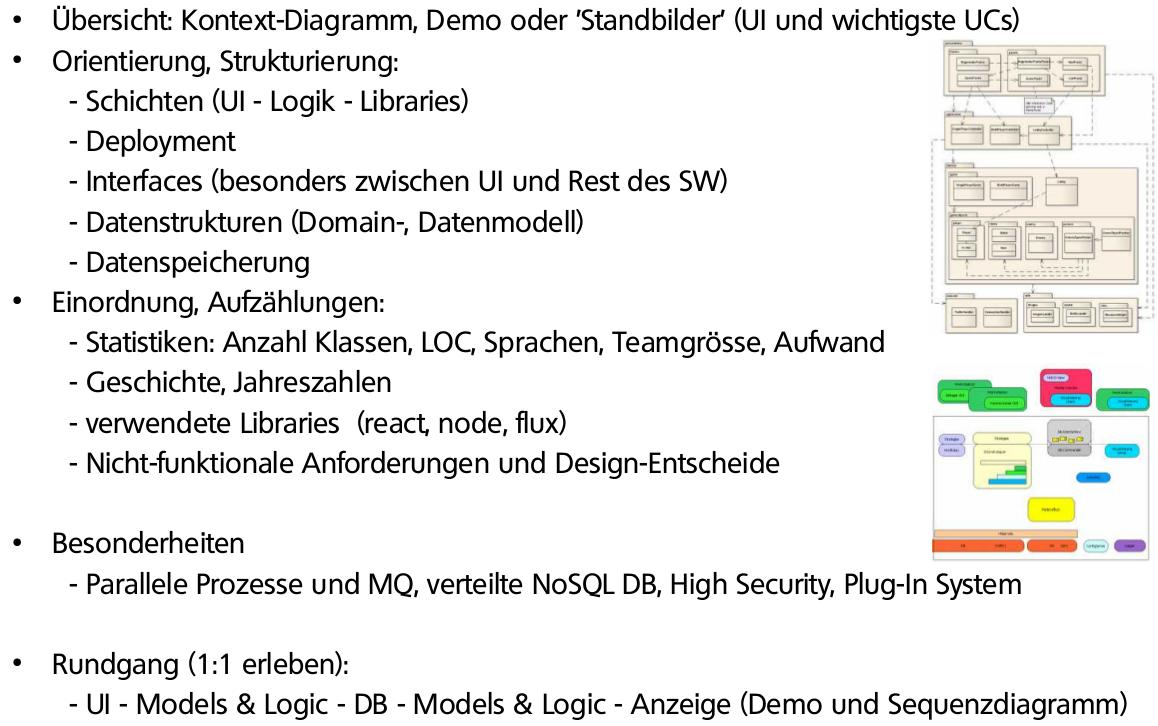
\includegraphics[width=0.7\linewidth]{img/architektur_praesentation}
	\caption{Architektur-Präsentation}
	\label{fig:architekturpraesentation}
\end{figure}

\subsection{Architektur-Überlegungen}
System-übergreifende Überlegungen (Cross-cutting concerns):
\begin{itemize}
	\item Fehlerbehandlung, Exception handling
	\item Logging (spannend wenn über mehrere Maschinen hinweg)
	\item Transaction handling
	\item Internationalisierung
	\item Backup, Löschen von Überflüssigem, z.B. Log-Entries in DB
	\item Deployment
\end{itemize}

Qualität:
\begin{itemize}
	\item Performance-Überlegungen (Mengen, Zeit, Geschwindigkeit), eventuelle Real Time and Space constraints
	\item Security/Safety-Überlegungen
	\item andere Qualitäts-Überlegungen (Erweiterbarkeit, Plattform-Portabilität, Verfügbarkeit...)
\end{itemize}

Analyse zu den Requirements:
\begin{itemize}
	\item Beschreibung der umliegenden Systeme und Aktoren, Schnittstellen
	\item Datenmodellierung (statisch, "was merken wir uns?")
	\item Prozessbeschreibungen (dynamisch, "was läuft ab?")
	\item Randbedingungen (IT Landschaft, politisch, juristisch)
	\item Nutzer, Rollen \& Rechte
	\item Vorgaben zu Security, Performance, Usability, Portability...
	\item UX-Vorgaben (oft Browser; besonders wichtig bei iOS/Android)
\end{itemize}


\subsubsection{Bausteine zur Beschreibung}

\begin{itemize}
	\item Context Diagramm (informelle und ausführlichere Darstellung von Aktoren und deren Interaktion)
	\item Schnittstellen zu Umsystemen
	\item Use Case Diagramm
	\item Prozessbeschreibung: Aktivitätsdiagramm (Detaillierte Beschreibung von Prozessen)
	\item Deployment-Diagramm
	\item Schichten-Architektur (packages)
\end{itemize}

\subsubsection{Technische Architektur-Entwurfsmuster}

\begin{itemize}
	\item Single User Desktop Program (Einfache, lokale Programme)
	\item Multi-Tier Architectures (Skalierbarkeit, Performance. Sehr komplex)
	\item Fat Client + Server (grosse Desktop-Programme und Mobile Apps)
	\item Thin Client (Browser Based + Server)
	\item DB-zentrierte Architektur  (Skalierbar, einfacher Aufbau, aber stark von DB abhängig)
	\item Produzent $\rightarrow$ Konsument (Konsument muss schneller sein als Produzent)
	\item Message Basierte Systeme (Skalierbarkeit, Performence, aber komplex)
\end{itemize}

\paragraph{Bei Multi-Prozess-Architektur}

müssen folgende Punkte sorgfältig definiert werden:

\begin{itemize}
	\item stateful/stateless
	\item singlethreaded/multithreaded
	\item Anfrage \& Antwort: asynchron/synchron (pro Anfrage)
	\item first-in/first-out oder priority queue
	\item point-to-point oder multipoint/broadcast communication
\end{itemize}

\subsubsection{Enterprise Integration Patterns}

Diagramm-Details sind nicht Prüfungsrelevant

\subsection{Software Architektur Dokumentation}

Beschreiben, wie das System aufgebaut wurde und warum das so gemacht wurde.

Die Doku hat zwei Hauptteile:
\begin{itemize}
	\item Umfeld und Randbedingungen
	\item Technische Struktur
\end{itemize}

\paragraph{Struktur:}

\begin{enumerate}
	\item Dokumentation Umfeld
		\begin{itemize}
			\item Context Diagram: Übersichtsbild, wichtig: die umliegenden Systeme und Aktoren
			\item IT-Landschaft mit Schnittstellen zu anderen Systemen
			\item Beschreibung der Datenhoheit in anderen Systemen: wo werden die Daten 'geboren', wo ist der 'single point of truth'
			\item Beschreibung der Aktoren, Rollen und Rechte
			\item Business Process Modelling
			\item Randbedingungen (juristisch, historisch ...)
			\item (Referenz zu Use Cases mit Use Case Diagramm)
			\item (Referenz zu Domainmodell)
			\item (Referenz zu nicht-funktionalen Anforderungen)
		\end{itemize}
	\item Dokumentation Technische Struktur
		\begin{itemize}
			\item Deployment diagram (was läuft wo), oft verschiedene Deployment-Szenarien, (meist sehr high-level)
			\item Schichten-Architektur, UML top level package/class diagram (was auf eine A3-Seite passt), zeigt, wie die Klassen/Pakete strukturiert sind.
			\item Datenmodell: UML class diagram oder E-R Diagramm.
			\item Bei den Beschreibungen v.a. auch auf die Assoziationen achten.
			\item Zustandsdiagramme/Lebenszyklen der wichtigsten Entitäten
			\item Prozesse, Threads mit ihren Charakteristiken; Message Queues
			\item UX Skizzen, Personas \& Szenarien, Screen shots, Erklärungen
		\end{itemize}
	\item Zoom: Technische Details mit Kommentaren, warum.
		\begin{itemize}
			\item UML Klassendiagramm als Übersicht: nicht zu detailliert, oder dann 1:1			aus Code generiert (aber: "Welchen Sinn hat eine Landkarte im Masstab 1:1 ?" Zitat Umberto Eco)
			\item UML Klassendiagramm als Detailbeschreibung v. etwas Kompliziertem
			\item UML Zustandsdiagramme
			\item UML Sequenzdiagramme
			\item parallele Prozesse (UML?)
			\item Gut auch: wieder verworfene andere Lösungen, warum verworfen; wo ist welche Erweiterbarkeit/Anpassbarkeit eingebaut (config files, scripting extensions, strategy pattern) und warum
		\end{itemize}
	\item Zoom: Dynamik
		\begin{itemize}
			\item Prozesse, Threads mit ihren Charakteristiken; Prozess-Interaktion über Message Queues (z.B. JMS)
			\item UX Architektur (welche Screens folgen auf welche)
			\item Ablauf-Szenarien, z.B. Click - call - message - call - message, etc. (Sequenz-Diagramme)
			\item Data flows, Control flows (Aktivitäts-Diagramme)
		\end{itemize}
\end{enumerate}


\subsection{Architektur-Refactoring}

Bei schlechter Architektur, kann folgendermassen vorgegangen werden:

\begin{enumerate}
	\item Layering einführen/verbssern, so lange, bis es nur Zugriffe von oben nach unten gibt.
	\item Mittlere Schicht entwirren: Aufteilung von Business-Services und evtl. Domainklassen.
	\item Partitionieren und aufteilen von Klassen.
\end{enumerate}


\section{Scrum II}

Bei vorgehen nach Scrum gibt es nur einen gröberen Architekturplan 
Scrum funktioniert nur, wenn man sich an die zwingenden Voraussetzungen hält:

\begin{itemize}
\item Teamgrösse max. 10
\item kurzes Projekt max. 9 Monate
\item Kunde weiss noch nicht so genau, was er will
\item Ganzes Team an einem Ort
\item Team deckt alle Fähigkeiten ab
\item Häufige, mündliche Kommunikation
\item Kunde im Team, ständig verfügbar
\item Kunde will agiles Vorgehen
\end{itemize}

Bei gewissen Projekten bieten sich folgende Ergänzungen an:

\begin{itemize}
	\item Checkpoint End of Elaboration (wie im Unified Process)
	\item Zweite, höhere Abstraktionsstufe zu User Stories im Backlog
		\begin{itemize}
			\item Use Cases
			\item Szenarien
			\item Personas
			\item Domain Model
			\item Nicht funktionale Anforderungen
		\end{itemize}
	\item Zusätzliche Rolle des Projektleiters, für all das, was der Product Owner und das Team nicht abdecken
\end{itemize}

\subsection{Product Owner vs. Projektleiter}

Der Product Owner vertritt die Kundenseite.

Der Projektleiter ist z.a. für folgende Punkte verantwortlich:
\begin{itemize}
	\item Qualität und Testing
	\item Planung von z.B. Datenmigration, Datenverwaltung
	\item Umsetzungsentscheide bei Unstimmigkeiten
	\item Organisation
	\item Stunden und Rechnungen
\end{itemize}

\subsubsection{Projektleiter ohne technisches Verständnis}

Ist ein Projektleiter kein Entwickler, braucht er einen ''ersten Offizier'', welchem er blind vertrauen kann, und der sich sehr gut auskennt.

\subsection{Daily Standup}

Am Daily Standup dürfen nur aktiv am Projekt involvierte und arbeitende etwas sagen (''Pigs''). Am Rande Beteiligte dürfen zwar teilnehmen, aber nichts sagen (''Chicken'').

\subsection{Backlog}

Der Backlog braucht Pflege, sogenanntes ''Backlog Refinement'':

\begin{itemize}
	\item Schätzen
	\item Priorisieren
	\item Aufteilen
	\item Löschen
\end{itemize}

\subsubsection{Impediments}

Impediments (Hindernis) Tracking ist das äquivalent zum traditionellen Bug Tracking. Es dient in erster Linie dem aufzeigen von externen Abhängigkeiten / Blockaden

\subsection{MVP: Minimum Viable Product}

Bei Kunden, welche keine Entwickler sind, sollte bei jedem Sprint nach Möglichkeit eine sichtlich bessere Software herausfallen.

Bei Projekten, deren MVP sehr gross ist, funktioniert Scrum nicht. Bei Projekten, wo die Funktionen von vornherein 100\% klar sind, macht Scrum nur mässig Sinn.


\subsubsection{Fortschritt sichtbar machen}

\paragraph{Für den Kunden}
\begin{itemize}
	\item Burn-Down Chart
	\item Story Map mit Farben
	\item Trends (Bug Reports, build failures, Metriken, ... )
\end{itemize}

\paragraph{Für die Entwickler}
\begin{itemize}
	\item Backlog
	\item Metriken
	\item Testabdeckung
	\item SonarQube
\end{itemize}

\paragraph{Für die IT-Infrastruktur}
\begin{itemize}
	\item Dashboards mit Ressourcen-Verbrauch (Disk, CPU...)
	\item Log-Auswertungen visualisiert
\end{itemize}


\section{Proving Programs}

Mittels Unit Tests lässt sich nur die Anwesenheit von Bugs beweisen, aber nicht deren Abwesenheit. Deshalb ist ein interessanter Ansatz, Programme formal zu beweisen.

\subsection{Hoare Triples}

\[ \left\{P\right\} C \left\{Q\right\} \]

Wenn das Programm $C$ von einem Zustand ausgeführt wird, welche der Vorbedingung $P$ genügt, ist nach der Ausführung die Nachbedingung $Q$ erfüllt.

$P$, $Q$ und das ganze Hoare Triple sind dabei Prädikate. $P$ und $Q$ zeigen den Zustand des Programms mittels den Variablen in $C$ als freie Variablen.



\subsection{Automatisierung von Tests}

\subsubsection{if}

\begin{lstlisting}
{T}
{(x < 0 => -x >= 0) AND (not x < 0 => x >= 0)}
if x < 0 then
	{x >= 0}
	y := -x
else
	{x >= 0}
	y:=x
{y >= 0}
\end{lstlisting}

Resultiert in der verification condition: $\vdash (x<0 \implies -x \leq 0) \land (\lnot (x < 0) \implies x \leq 0)$

\subsubsection{while}

Ganz beweisen lassen sich while loops nicht (aufgrund des Halting Problems.)

Loop invariant ist eine Eigenschaft, welche immer am Ende einer loop wahr sein muss (d.h. sie bleiben gleich, bzw. ändern sich vorhersagbar).

Ein Loop invariant zu finden, kann nicht automatisch gelöst werden.


\begin{lstlisting}
{x >= 0}
{0 <= x}
i := 0;
{i<=x}
while NOT(i = x) do {Inv : i <= x}
	{i<=x ^ NOT(x=i)}
	{i+1 <= x}
	i := i + 1
	{i<=x}
{i <= x AND NOT (NOT(i = x))}
{i = x}
\end{lstlisting}

Wenn wir folgendes Beweisen können, ist die Loop invariant richtig:

\begin{align*}
\vdash & i \leq x \land x \neq i \implies i + 1 \leq x \\
\vdash & i < x \implies i+1 \leq x \\
\vdash & x -1
\end{align*}

Wir müssen dabei drei Beweisbedingungen beachten:
\begin{itemize}
	\item Ist es eine loop-variant \begin{itemize}
		\item Muss eine Bedingung sein, welche zwingend vorher und nachher (allgemein) gültig ist
	\end{itemize}
	\item kann ich mit der loop-invariant zur post-condition kommen
	\item kann ich von allen vorbedingung zur loop-invariant implizieren
\end{itemize}

Danach betrachten wir die Schlaufe als Blackbox; wir müssen nun implizieren, dass wir die letzte postcondition aus der Invariant herleiten können

\textit{Das finden von loop variant ist nicht prüfungsrelevant.}


\appendix

% Code Listings
\lstlistoflistings

% List of figures
\listoffigures

% List of tables
\listoftables

% Bibliography
\bibliographystyle{plain} 
\bibliography{literatur}

\end{document}
